\chapter{Requirements Analysis And application design}


\section{Existing Slutions}
In this subsection i will focus on studying some applications which have the same context as my project in order to retain some of  the helpful features proposed by these applications and avoid their drawbacks. 
\subsubsection{CNN NEWS APPLICATION }

\begin{figure}[h!]
	
\includegraphics[width=13cm]{image3.png}
	\caption{Logo OF CNN NEWS }
	\label{cnn logo}
\end{figure}
\begin{enumerate}
  \item Description of the application:
  \begin{description}
  
  \item \underline{Application name:} CNN Breaking US And World News
  \item \underline{Description:}CNN app is   a portal to the latest breaking news  from around the globe   
  \item \underline{App version:}  2.9.4
  \item \underline{Last updated:}  july , 18 , 2016 
  \item \underline{App size:}  40M
  \item \underline{Offered by:} CNN
  \item \underline{Rate:}  4 stars 
   
\end{description}

  \item Criticism of the application :
  
\begin{itemize}
\item Positive points:
\begin{enumerate}
 \item \underline beautiful user interface (material design ) :Material design is a comprehensive guide for visual, motion, and interaction design across platforms and devices . It's is highly recommended to use in android apps since it's is supported by android devices .
 
 	 	
\begin{figure}[H]
 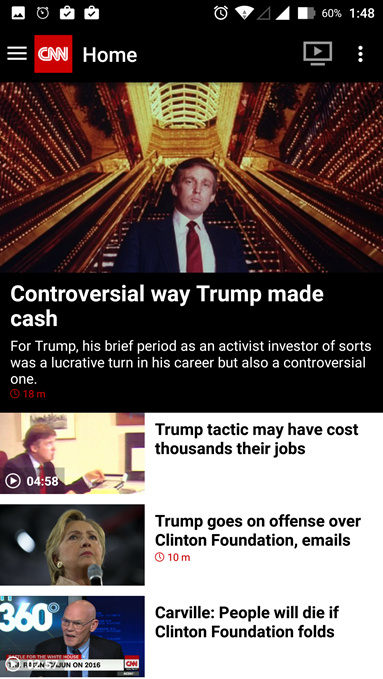
\includegraphics[width=10cm]{cnn_design.png}
 \caption{CNN UI}
	\label{france24 UI}
\centering
\end{figure}
	


 
 \item Giving the choice to the user to choose wether to receive push notification or not : this step helps to improve the ux (user experience) of the app .
 

\begin{figure}[H]
	
\includegraphics[width=10cm]{cnn_push.png}
	\caption{CNN push notifications}
	\label{CNN push notifications}
\centering
\end{figure}
	

 
 

	

\end{enumerate}  
  
  
 \item Drawbacks: 
 \begin{enumerate}
 \item big size : 40M
  \end{enumerate}  
\end{itemize}  
\item Proposed Solutions And Retained Features :
\\* 
From all the previous features i will retain all the positive ones and i will try to avoid all the drawbacks .  
\\*
so to summarize the product must present these features:  
\begin{itemize}
\item beautiful material  design  
\item speed and performing application 
\item light weight app 
\item giving the user the choice whether to receive push notifications or not
\end{itemize}


\end{enumerate}
 \newpage
 \subsubsection{FRANCE 24}
\begin{figure}[h!]
	
\includegraphics[width=7cm]{france24.png}
	\caption{Logo of France 24  }
	\label{france24}
\end{figure}
	
\begin{enumerate}
  \item Description of the application:
  \begin{description}
  
  \item \underline{Application name:} France 24 
  \item \underline{Description:} France 24 mobile app is an application which will keep up to date with international news .   
  \item \underline{App version:} varies with device 
  \item \underline{Last updated:} August 9, 2016  
  \item \underline{App size:}  varies with device but big anyway 
  \item \underline{Offered by:} France Médias Monde
  \item \underline{Rate:}  4.2 stars 
   
\end{description}

  \item Criticism of the application :
  
\begin{itemize}
\item Positive points:
\begin{enumerate}
 \item \underline Breaking news popups when the app is in foreground . 


 	
\begin{figure}[H]
 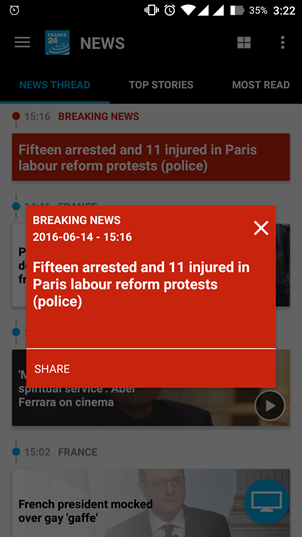
\includegraphics[width=10cm]{france24_popup.png}\caption{France popup}
	\label{france24 poopup}
\centering
\end{figure}
 
 
 \item \underline Push notifications : 
 \\*
 \\*
   \begin{figure}[H]

\includegraphics[width=10cm]{france24_push.png}\caption{France push notifications }
	\label{france24 notifications}
\centering
\end{figure}
 

  \item \underline Beautiful UI .

  
  \begin{figure}[H]
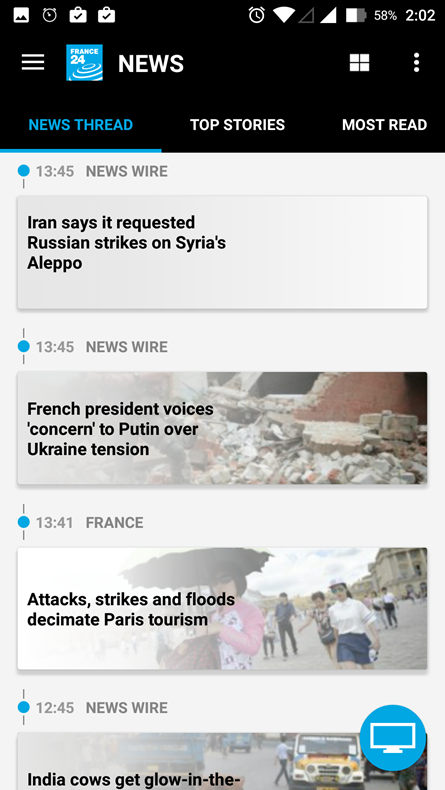
\includegraphics[width=10cm]{france24_ui.png}
\caption{France 24 UI }
	\label{france24 ui}
\centering
\end{figure}
 
\end{enumerate}  
  
  
 \item Drawbacks: 
 \begin{enumerate}
 \item big size 
  \end{enumerate}  
\end{itemize}  
\item Proposed Solutions And Retained Features :
\\* 
From all the previous features i will retain one feature which is the manner how the posts are designed to show with a little modification .


\end{enumerate}
 \newpage
 
 \subsubsection{ASSABAH NEWS : }


\begin{figure}[H]
	
\includegraphics[width=7cm]{assbah.jpg}
	\caption{Logo of assabah news }
	\label{imag3}
\end{figure}
\begin{enumerate}
  \item Description of the application:
  \begin{description}
  
  \item \underline{Application name:} Assabah News 
  \item \underline{App version:} 1.0
  \item \underline{Last updated:} October 10, 2014
  \item \underline{App size:}  :  2.9M
  \item \underline{Offered by:} Orange tunisie 
  \item \underline{Rate:}  4.2 stars 
   
\end{description}

  \item Criticism of the application :
  
\begin{itemize}
\item Positive points:
\\* 

light weight app
 
  
  
 \item Drawbacks: 
\\the ui is not very beautiful

\begin{figure}[H]
	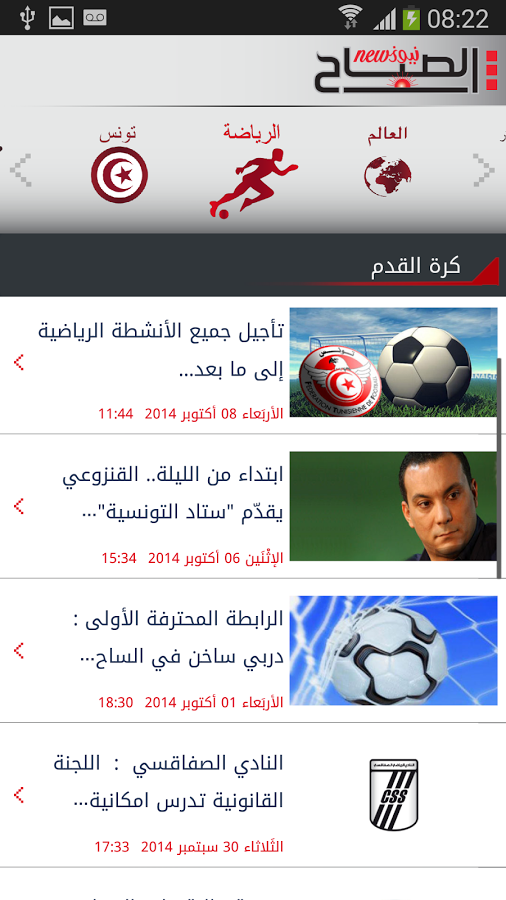
\includegraphics[width=7cm]{assabah_news.png}
	\caption{Assabah news UI }
	\centering
	\label{imag3}
\end{figure}
  
\end{itemize}  
\item Proposed Solutions And Reatained Features :
\\* 
From all the previous features i have been impressed by the little size of the application that's why i will try to make it lightweight as possible .

\end{enumerate}

\section{Requirements Analysis}


\subsection{Informal Requirements Analysis}

\subsubsection{Functional Requirements Analysis}

\begin{itemize}
\item Functionalities:

\begin{itemize}
\item browse news divided by main categories : politique ,  economie , ... (vertical navbar ) , and small categories : ce que je pense ,  (horizontal navbar) .
\item Integrate push notifications service in the app and in the website by developing a WordPress  plugin (php code ) 
\end{itemize}

\item Project Dependencies  : 
\begin{itemize}
\item 	The application must communicate with the website database by using the plugin which must be installed on the WordPress website .
\item The push notification service must communicate with  google servers since we are using the google cloud messaging (GCM)  for push notifications . And then the servers responds with a registration id  which will be sent to the plugin which will insert it in the website?s database to use it later when sending the push notifications  
\end{itemize}

\end{itemize}

\subsubsection{Non Functional Requirements}


\begin{itemize}
\item 	Code must be clear and  commented for future evolutions . 
\item 	Ergonomics : the application must  have a friendly and easy to use UI.
\item  Security : the application must respect the confidentiality of data .
\item 	Ensure the integrity and consistency of data in each update, and each insertion .
\item 	Portability : the plugin must work with every WordPress website , and the app must be generic as much as possible 
 
\end{itemize}

\subsection{Semi-formal Requirements Specification }


\begin{itemize}
\item use case diagrams :

\begin{itemize}
\item browse news :
\begin{figure}[h!]
	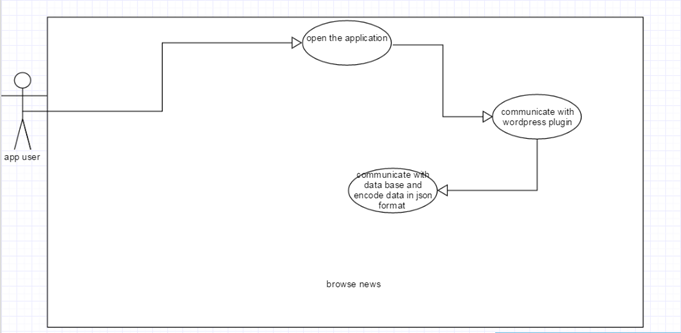
\includegraphics[width=13cm]{usecase1.png}
	\caption{Browsing news use case}
	\label{imag3}
\end{figure}
\item push notification :
 \begin{figure}[h!]
	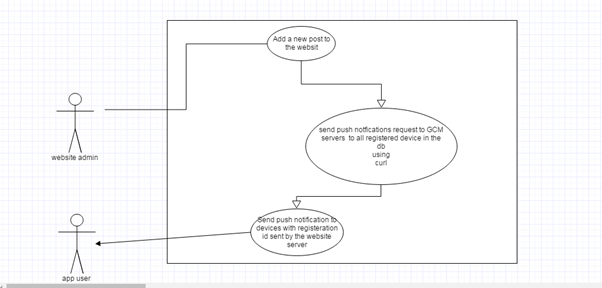
\includegraphics[width=13cm]{usecase3.png}
	\caption{Push notification use case diagrams}
	\label{imag3}
\end{figure}
\end{itemize}
\item	Presentation of actors :
\begin{itemize}
\item App user : the user of the app 
\item Website admin : the person or the group of persons who are responsible for updating the database or postings new news on the website .

\item  Browse news : the actor opens the app the app will send AJAX request to the plugin . The purpose of these requests is asking for receiving data using json format . then the wordpress plugin which is already connected to the database selects the suitable data using the category name to select it right and then it encodes the data retrieved and responds the ajax call with the required data in JSON format .
\item Push notification : the website admin adds a new post on the site invokes the sending of curl request to GCM servers for each device registered on the site . and finally the GCM servers sends push notifications to these devices or updates the app if it?s in foreground .
\end{itemize}

\end{itemize}

\subsection{Application design}
\subsubsection{Sequence diagrams}
\begin{itemize}
\item \textbf{Data extraction sequence diagram:}
 	 	
\begin{figure}[H]
 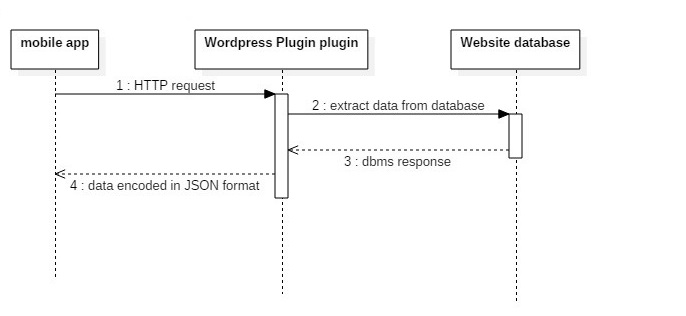
\includegraphics[width=10cm]{sequence2.jpg}
 \caption{Data extraction sequence diagram}
	\label{Data extraction sequence diagram}
\centering
\end{figure}
	
\item \textbf{plugin sequence diagram:}
\begin{figure}[H]
 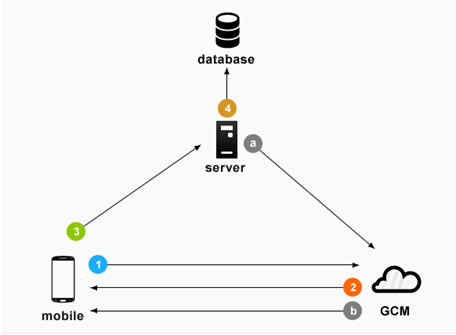
\includegraphics[width=10cm]{sequence1.png}
 \caption{Data extraction sequence diagram}
	\label{Data extraction sequence diagram}
\centering
\end{figure}
\item \textbf{Push notification squence diagram:}

\begin{itemize}
\item Push notification squence diagram : 
 \begin{figure}[h!]
	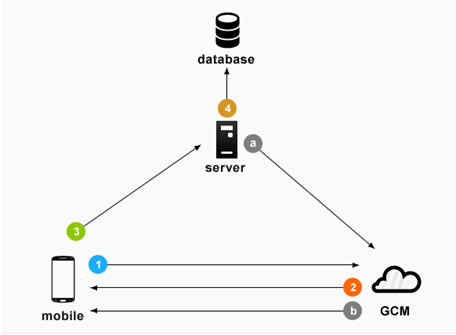
\includegraphics[width=13cm]{sequence1.png}
	\caption{Push notifications sequence diagram}
	\end{figure}
\item Description :
\\*  
\\1. First android device sends sender id, application id to GCM server for registration. 
\\*
\\2. Upon successful registration GCM server issues registration id to android device. 
\\*
\\3. After receiving registration id. device will send registration id to our server 
\\*
\\4. Our server will store registration id in the database for later usage 
\\*
\\(a) Whenever push notification is needed, our server sends a message to GCM server along with device registration Id (which is stored earlier in the database)
\\*
\\(b) GCM server will delayers that message to respected mobile device using device registration id 
\end{itemize}
\end{itemize}

\subsubsection{UI Design}
 To have an idea ,about how the UI of the app will be , i have deisgned some interfaces using adobe photoshop :
 \begin{itemize}
 \item Home Screen
 

 
\begin{figure}[H]
\centering
 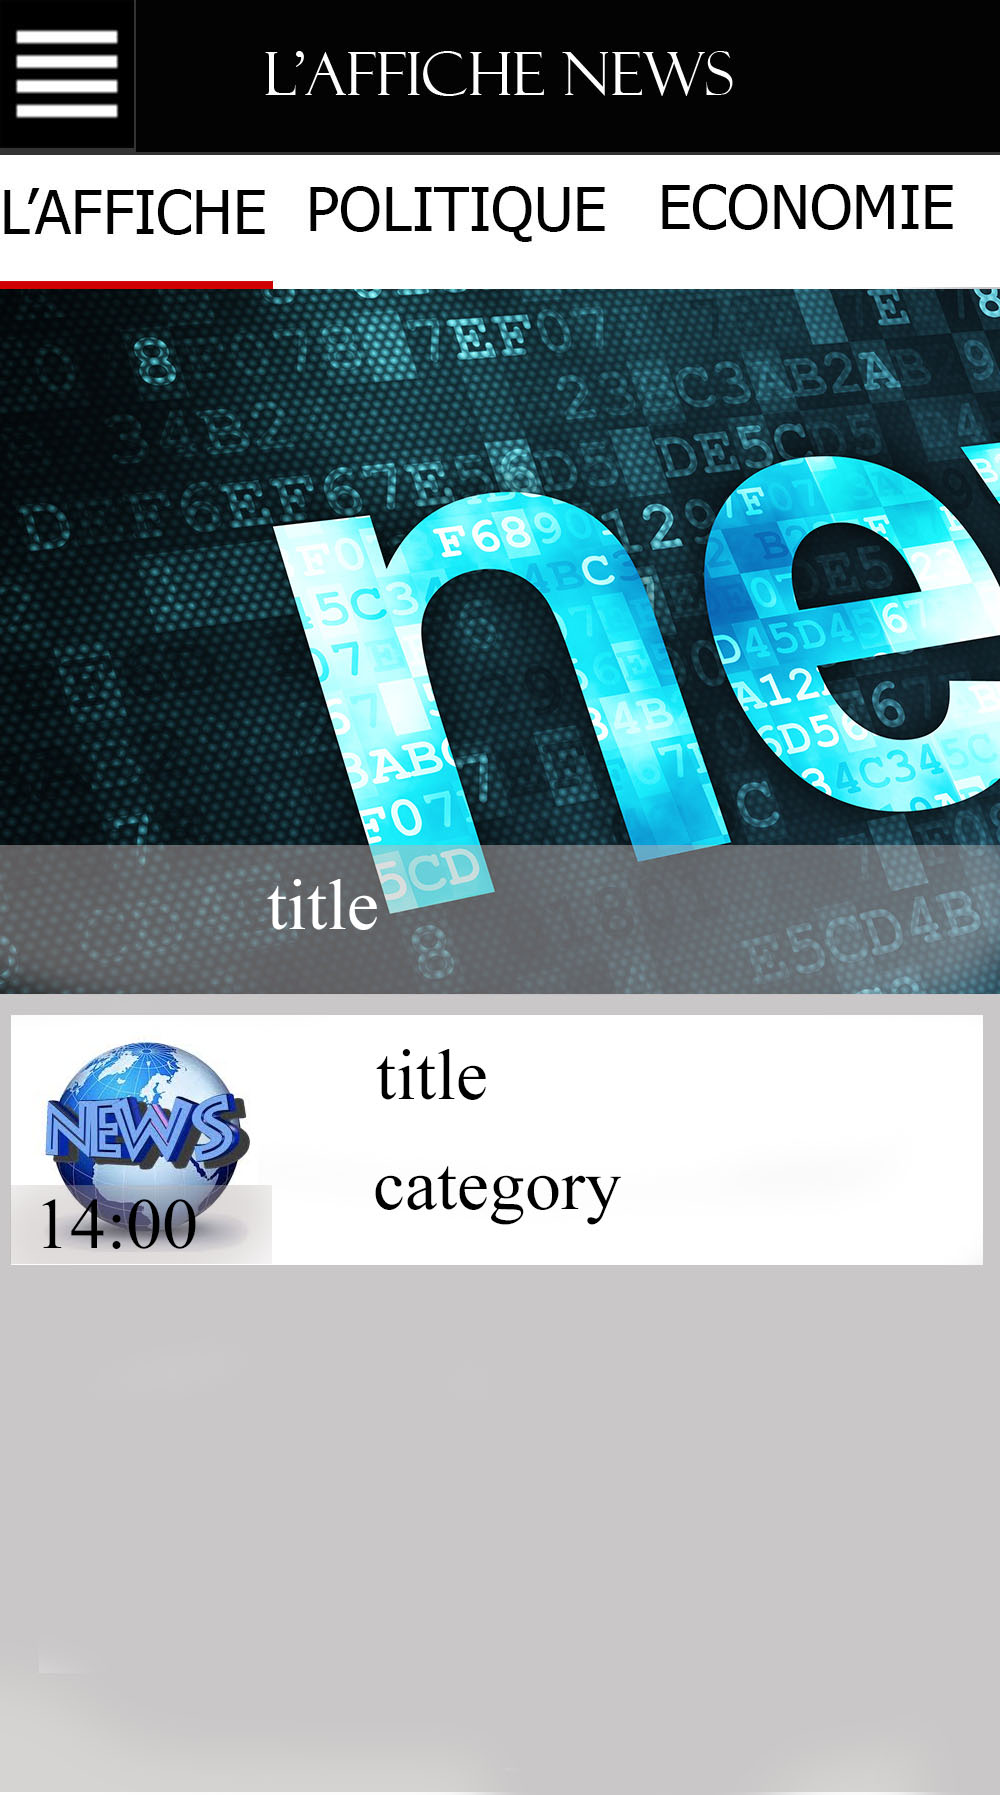
\includegraphics[width=6cm]{home_screen.jpg}
 \caption{Home screen UI}
 
	\label{home screen ui}

\end{figure}
\item Slide out menu :
 \begin{figure}[H]
\centering
 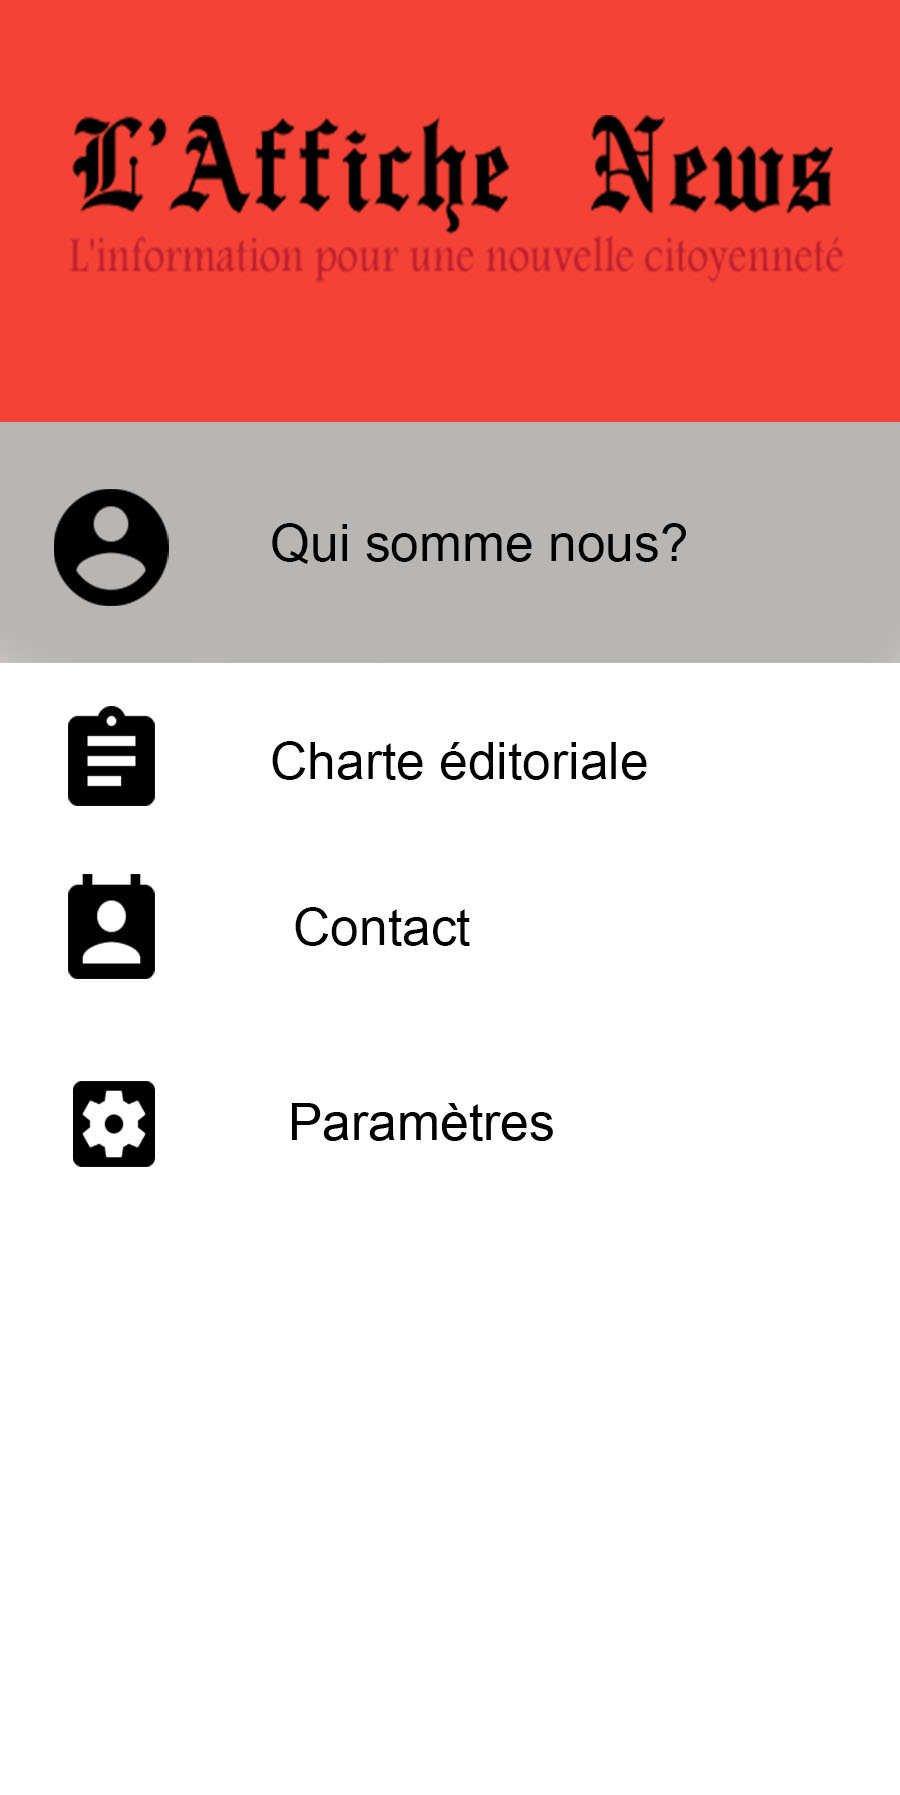
\includegraphics[width=6cm]{slide_out.jpg}
 \caption{Slide Out menu}
 
	\label{slide out menu}

\end{figure}
 \end{itemize}

\textbf{Note:} You may notice some differences between these interfaces and the actual application design because of updates and new ideas during the developement
